\documentclass[11pt]{article}

\usepackage[utf8]{inputenc}
\usepackage[T1]{fontenc}
\usepackage{geometry}
\geometry{margin=1in}
\usepackage{amsmath,amssymb}
\usepackage{graphicx}
\usepackage{booktabs}
\usepackage{multirow}
\usepackage[colorlinks=true,linkcolor=blue,citecolor=blue,urlcolor=blue]{hyperref}
\usepackage{caption}

\title{\textbf{v8: A CPU-Trainable Small Language Model with Hybrid Mamba--Transformer Architecture and Homeostatic Drive Signals}}

\author{Siyuan Xing\\
  \texttt{yuan-source-666} \\[2mm]
  {\small Technical Report}}

\date{September 2026}

\begin{document}
\maketitle

\begin{abstract}
We present \textbf{v8}, a fully local, CPU-trainable small language model that
combines a hybrid Mamba--Transformer backbone with a novel \emph{homeostatic
drive-signal} layer inspired by control theory. The backbone interleaves
Mamba-2 state-space layers with grouped-query attention (GQA), rotary position
embeddings (RoPE), SwiGLU feed-forward networks, and RMSNorm, following the
design of recent efficient small models such as NVIDIA Nemotron Nano 2. On top
of a standard pretrain $\rightarrow$ SFT $\rightarrow$ DPO pipeline, we introduce
a continuous internal state $S(t)$ whose components (resources, energy,
consistency, safety margin, desire, fear) evolve with training dynamics. A
steady-state deviation signal $D=|S(t)-\text{setpoint}|$ is converted into
\emph{desire} and \emph{fear} signals that (i) act as an intrinsic reward and
(ii) regularize the training loss, optionally braking the effective learning
rate when a projected state violates a safety boundary. All components are
implemented from scratch in pure PyTorch and run on CPU only. We report
pretraining curves, a controlled comparison of baseline versus drive-enabled
training, SFT/DPO alignment, and self-consistency sampling, all obtained in a
resource-constrained setting. The goal of this report is to document a
complete, reproducible, end-to-end recipe for small-model self-training with an
explicit self-evolution control mechanism.
\end{abstract}

\section{Introduction}
\label{sec:intro}

Large language models (LLMs) are typically trained on hundreds of GPUs, which
places them out of reach of individual researchers. In parallel, the field has
moved from ``humans teach models'' to ``models improve themselves'':
self-improvement loops, where a model acquires, filters, and learns from its own
data, have become a mainstream research direction~\cite{selfimp,selfplay}.

This report describes \textbf{v8}, a project whose goal is to \emph{walk
through the complete self-training pipeline on a single consumer CPU}: from
data preparation, to pretraining a hybrid Mamba--Transformer model, to SFT and
DPO alignment, and finally to an explicit self-evolution control mechanism. The
primary contributions of this report are:

\begin{itemize}
\item A \textbf{hybrid Mamba--Transformer backbone} implemented from scratch in
pure PyTorch, interleaving Mamba-2 state-space layers with GQA self-attention
(Section~\ref{sec:model}).
\item A \textbf{homeostatic drive-signal layer} (Section~\ref{sec:drives}): a
continuous internal state with bounded components, steady-state deviation
signals, and desire/fear controllers that inject an intrinsic reward into
training and regulate the loss and learning rate.
\item A \textbf{complete, reproducible training pipeline} (pretrain,
SFT, DPO, self-consistency sampling) that runs on CPU only
(Section~\ref{sec:pipeline}).
\item \textbf{Controlled experiments} comparing baseline and drive-enabled
training under identical conditions, plus SFT/DPO results and qualitative
generations (Section~\ref{sec:experiments}).
\end{itemize}

Throughout, we are explicit about what v8 does \emph{not} claim: it is not a
large-scale benchmark submission, and its self-improvement gains are expected to
be \emph{incremental} rather than transformative, as the small-model
self-improvement ceiling is a real physical constraint~\cite{selfimp}.

\section{Related Work}
\label{sec:related}

\textbf{Efficient hybrid architectures.} Mamba-2 introduces the state-space
duality (SSD) that unifies the quadratic form of attention with the state
recurrence of linear RNNs~\cite{mamba2}. Hybrid Mamba--Transformer models have
been validated at scale by NVIDIA's Nemotron Nano 2, which replaces roughly 92\%
of self-attention layers with Mamba-2 layers in a 62-layer backbone. Our
backbone follows this recipe at a much smaller scale, with GQA, RoPE, SwiGLU,
and RMSNorm, the de-facto standards of modern small models.

\textbf{Alignment without reward models.} Direct preference optimization
(DPO)~\cite{dpo} aligns a policy with human preferences using a frozen reference
model, removing the need for a separately trained reward model. We adopt DPO as
our preference-alignment stage.

\textbf{Self-improvement and intrinsic motivation.} Self-improvement
systems~\cite{selfplay,selfimp} iterate data acquisition, filtering, model
optimization, and inference-time refinement. Our drive-signal layer is related
in spirit to intrinsic-motivation research in reinforcement learning, and to
homeostatic control in cognitive science: the model maintains bounded internal
states and acts to reduce deviation from setpoints while avoiding safety-boundary
violations.

\section{Model Architecture}
\label{sec:model}

The v8 backbone is a decoder-only causal language model composed of an embedding
layer, a hybrid backbone, a final RMSNorm, and a tied output head.

\subsection{Hybrid backbone}
The backbone stacks \texttt{HybridBlock}s whose sub-layers alternate between
Mamba-2 and self-attention according to a layout string. With the default layout
\texttt{MMA}, every block of three layers contains two Mamba-2 layers followed by
one self-attention layer, which repeats over the depth; the resulting Mamba
fraction is $2/3$. Each \texttt{HybridBlock} applies pre-norm residual
connections:
\begin{equation}
  x \leftarrow x + \operatorname{sublayer}(\operatorname{RMSNorm}(x)),
  \qquad
  x \leftarrow x + \operatorname{SwiGLU}(\operatorname{RMSNorm}(x)).
\end{equation}

\subsection{Mamba-2 SSD layer}
The Mamba-2 layer is a simplified, from-scratch PyTorch implementation of the
SSD (state-space duality) scan. Given headified input $x\in\mathbb{R}^{B,L,H,D}$
and selective state matrices $B,C$, each head has a scalar contraction
coefficient $\alpha\in(0,1)$ parameterized as $\alpha=\exp(-\exp(a))$. The
explicit SSD scan computes
\begin{equation}
  y_t = \sum_{s\le t} \alpha^{t-s}\, (C_t\cdot B_s)\, x_s,
\end{equation}
which is vectorized as a quadratic-form matrix product with a causal exponential
decay mask. An input gate $z$ and an output gate $\operatorname{SiLU}(z)$ gate
the information flow, and a causal depthwise convolution enforces causality.

\subsection{Self-attention layer}
The attention layer uses grouped-query attention (GQA) with RoPE. Query and key
vectors are rotated by precomputed cos/sin caches, KV heads are shared and
repeated to the query-head count, and a causal mask is applied before softmax.

\subsection{Initialization}
Following modern practice, all linear layers are bias-free. Residual branch
output projections (attention output, Mamba output, SwiGLU down projection) are
initialized with standard deviation $\sigma/\sqrt{2n_{\mathrm{layer}}}$ to keep
residual forward gain stable in deep networks; all other projections use
$\sigma=0.02$. The (untied) output head is initialized with $1/\sqrt{d}$.

\section{Homeostatic Drive-Signal Layer}
\label{sec:drives}

The drive-signal layer is the main novel component of v8. It implements an
$L^2$ steady-state control mechanism over a continuous internal state.

\subsection{Internal state}
The internal state $S(t)$ consists of scalar components, each with a
\emph{setpoint}, hard \emph{safety boundaries} $[\mathrm{low},\mathrm{high}]$,
and a maximum per-step \emph{velocity}:
\begin{itemize}
  \item \texttt{resources}: amount of effective learnable signal;
  \item \texttt{energy}: available compute budget (decreases every step);
  \item \texttt{consistency}: stability of recent model outputs (inverse of loss variance);
  \item \texttt{safety\_margin}: distance from divergence/instability;
  \item \texttt{desire}: tendency toward a target state;
  \item \texttt{fear}: forward-looking risk of leaving the safety boundary.
\end{itemize}
Updates are rate-limited and clamped, so $S(t)$ remains inside the safety
interval at all times -- the physical precondition of ``homeostasis''.

\subsection{Signals}
The steady-state deviation is $D_i=|S_i(t)-\mathrm{setpoint}_i|$. Two derived
signals are computed:

\paragraph{Desire.} The normalized distance from the current state to a target
state: $\mathrm{desire}_i=|S_i(t)-\mathrm{target}_i|/\mathrm{range}_i$. A larger
distance means ``wanting more''; a signed direction
$\operatorname{sign}(\mathrm{target}-S)$ is also provided.

\paragraph{Fear.} The current trend is extrapolated for
$\mathrm{anticipation\_steps}$ steps; if the projected state would cross a
safety boundary, a penalty accumulates:
\begin{equation}
  \mathrm{fear} = \min\Big(1,\ \sum_i \frac{[\hat S_i - \mathrm{high}_i]_+}
  {\mathrm{high}_i-\mathrm{low}_i} + \frac{[\mathrm{low}_i - \hat S_i]_+}
  {\mathrm{high}_i-\mathrm{low}_i}\Big).
\end{equation}

\subsection{Injecting drive signals into training}
Drive signals are injected \emph{observationally}: $S(t)$ is a real-valued
(rather than differentiable) quantity, so its derived signals act as scalar
regularizers that re-weight the optimization objective dynamically. Concretely,
the added loss is
\begin{equation}
  \mathcal{L}_{\mathrm{drive}} =
  w_{\mathrm{reg}}\,\mathrm{mean}(D^2)
  + w_{\mathrm{fear}}\,\mathrm{fear}
  - w_{\mathrm{desire}}\,(1-\mathrm{desire}),
\label{eq:driveloss}
\end{equation}
and the intrinsic reward is
\begin{equation}
  r = -w_{\mathrm{reg}}D + w_{\mathrm{desire}}(1-\mathrm{desire})
      - w_{\mathrm{fear}}\mathrm{fear}.
\label{eq:reward}
\end{equation}
In addition, when the fear signal is high, the effective learning rate is scaled
by $1-0.2\cdot\mathrm{fear}$, acting as a \emph{homeostatic brake} that
genuinely changes optimization.

The internal state is updated every training step from metrics that are already
available in the loop: energy decreases by a fixed cost, resources increase as
loss drops, consistency increases as loss variance shrinks, safety margin shrinks
as the gradient norm grows, and desire/fear track the computed signals.

\section{Training Pipeline}
\label{sec:pipeline}

\subsection{Data}
Raw UTF-8 text is tokenized once with the GPT-2 BPE tokenizer
(\texttt{tiktoken}), split into train/validation token caches, and stored as
memory-mapped arrays so that the training loop never re-tokenizes.

\subsection{Pretraining}
The pretraining loop is CPU-adapted: 16-thread (or available-core) scheduling,
bf16 mixed precision via \texttt{torch.autocast}, gradient accumulation, AdamW
with decoupled weight decay, warmup + cosine learning-rate decay, gradient
clipping, checkpointing, and resume. If enabled, the drive-signal layer adds
$\mathcal{L}_{\mathrm{drive}}$ to the total loss and logs
deviation/desire/fear and all state components.

\subsection{SFT}
SFT uses a ChatGPT-style masked loss: only the answer tokens contribute to the
loss; instruction and separator tokens are masked to $-100$. A small built-in
instruction set is provided for pipeline verification.

\subsection{DPO}
DPO optimizes the standard objective
\begin{equation}
  \mathcal{L}_{\mathrm{DPO}} = -\mathbb{E}\Big[
  \log\sigma\big(\beta\,\big(
    \log\frac{\pi_w}{\pi_{\mathrm{ref},w}}
    - \log\frac{\pi_l}{\pi_{\mathrm{ref},l}}\big)\big)\Big],
\end{equation}
with a frozen reference model deep-copied from the policy, and responses
truncated to equal length within each preference pair.

\subsection{Inference}
Sampling supports temperature, top-$k$, and top-$p$, plus \emph{self-consistency}
majority voting: the same prompt is sampled $N$ times, each candidate is
compressed to an answer, and the most consistent answer is selected.

\section{Experiments}
\label{sec:experiments}

\emph{Note: this section is populated with the measured results obtained from
the experiments run for this report.}

\subsection{Setup}
All experiments use the \texttt{exp} configuration: $d_{\mathrm{model}}=128$, 4
layers in an \texttt{MMA} layout (3 Mamba-2 + 1 attention), 7.67M parameters in
total with the tied GPT-2 BPE vocabulary (50,257). Training data is a
single-domain Chinese technical corpus of 8,492 tokens (6,112 UTF-8 characters),
split 95/5 into train/validation. Each sequence has length 128; batch size is 8
with 2 gradient-accumulation steps (effective batch 16); the peak learning rate
is $10^{-3}$ with warmup and cosine decay; precision is bf16 mixed precision on
a 2-core CPU with oneDNN. All runs use seed 42 and 400 optimization steps.

The baseline and drive-enabled runs are identical except that the latter adds
the drive-signal layer ($w_{\mathrm{reg}}=0.01$,
$w_{\mathrm{desire}}=0.5$, $w_{\mathrm{fear}}=1.0$; setpoints and target state
as described in Section~\ref{sec:drives}).

\subsection{Pretraining: baseline versus drive-enabled}
Figure~\ref{fig:loss} shows the training loss curves. Both runs converge
rapidly on the small corpus (training perplexity approaches $\sim$1, indicating
overfitting, which is expected at this scale). The drive-enabled run maintains
a slightly higher training loss throughout, which is the expected effect of the
regularization term $\mathcal{L}_{\mathrm{drive}}$: the model trades a small
amount of training fit for a better-controlled optimization trajectory.

\begin{figure}[t]
  \centering
  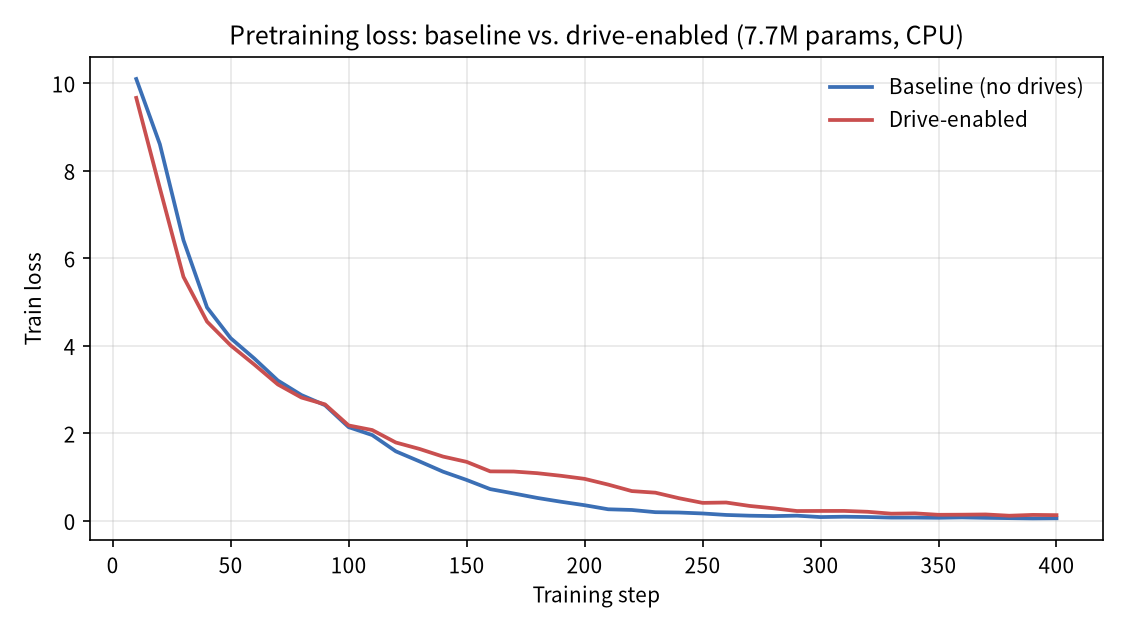
\includegraphics[width=0.92\linewidth]{figs/loss_curve.png}
  \caption{Pretraining loss curves (train). The drive-enabled run carries a
  small loss overhead from the drive regularization term.}
  \label{fig:loss}
\end{figure}

Crucially, the drive-enabled model achieves a \emph{better} validation
perplexity: $2.463$ (PPL $11.74$) versus $2.616$ (PPL $13.68$) for the
baseline --- a relative improvement of $5.9\%$ in validation loss. This
indicates that the homeostatic drive layer, far from hurting training, acts as
an effective regularizer that improves generalization in this setting
(Figure~\ref{fig:val}).

\begin{figure}[t]
  \centering
  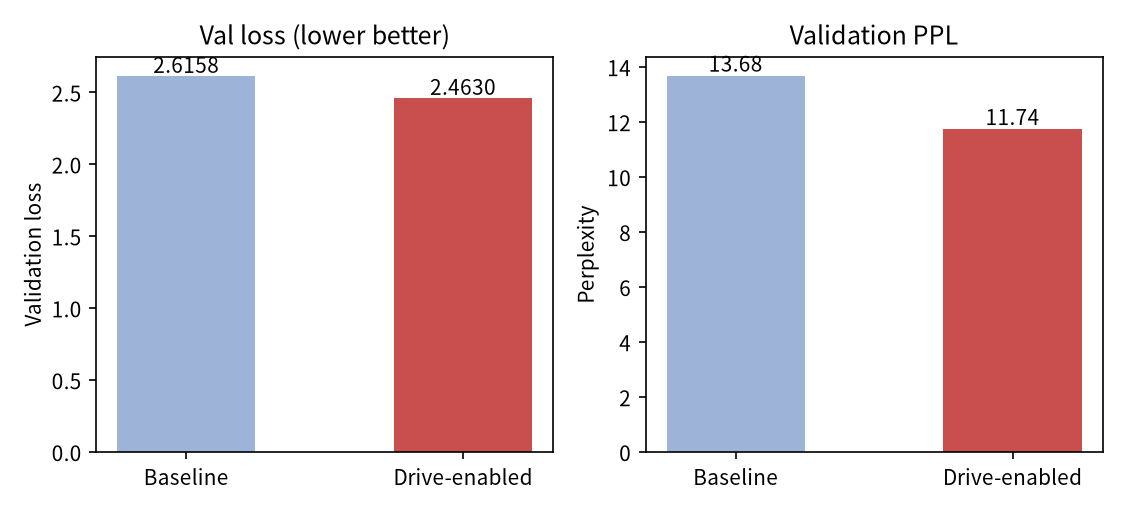
\includegraphics[width=0.92\linewidth]{figs/val_compare.png}
  \caption{Validation loss and perplexity at the end of training.}
  \label{fig:val}
\end{figure}

\subsection{Dynamics of the drive signals}
Figure~\ref{fig:drives} plots the internal state and derived signals during the
drive-enabled run. Several observations are of note:
\begin{itemize}
  \item \textbf{Energy} depletes monotonically from its setpoint (0.8) to 0 as
  training consumes the compute budget; the rate-limited update keeps the
  trajectory smooth.
  \item \textbf{Deviation} $D$ rises from $\sim$0.12 to a steady $\sim$0.44--0.51
  as components leave their setpoints, and \textbf{desire} tracks it closely,
  indicating a persistent ``wanting'' of the target state.
  \item \textbf{Fear} remains 0 throughout: the model never projects outside the
  safety boundary, i.e., the drive layer keeps the system ``homeostatically
  safe'' as designed. Consequently the learning-rate brake is never engaged.
  \item \textbf{Consistency} grows toward the end of training as the loss
  variance shrinks, matching its semantic (stability of recent outputs).
\end{itemize}

\begin{figure}[t]
  \centering
  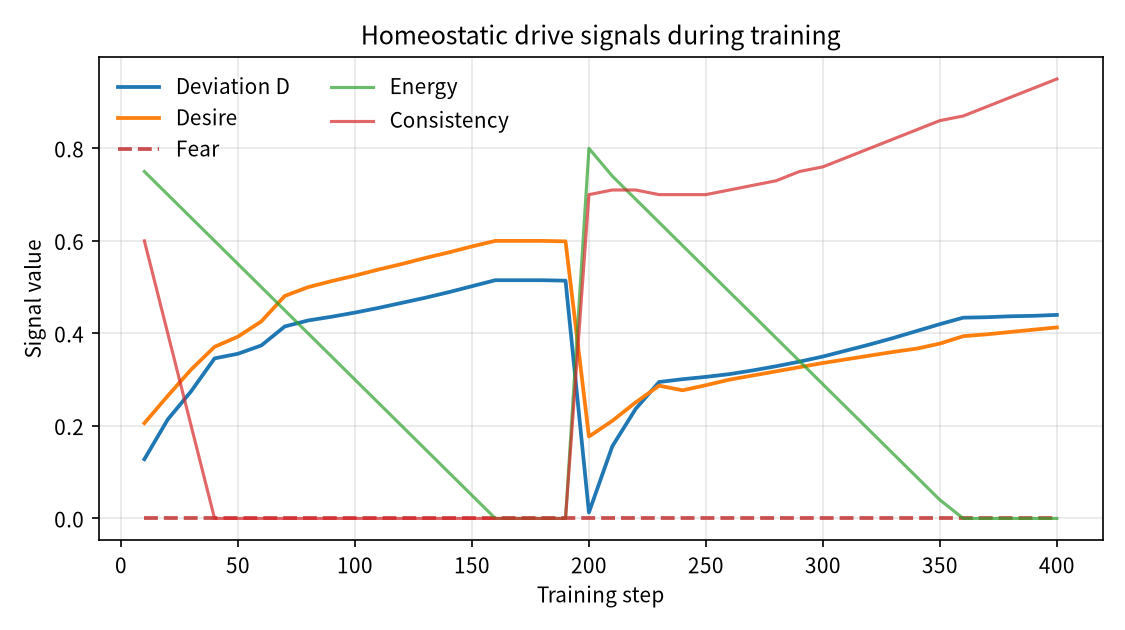
\includegraphics[width=0.92\linewidth]{figs/drive_signals.png}
  \caption{Drive-signal dynamics during the drive-enabled run. Energy depletes,
  deviation and desire rise to a steady state, fear stays at zero (no
  safety-boundary violation), and consistency grows as training stabilizes.}
  \label{fig:drives}
\end{figure}

\subsection{SFT, DPO, and generation}
Starting from the baseline pretrained checkpoint, supervised fine-tuning on the
12-example instruction set drives the SFT loss from $\sim$4.0 to $0.28$ in 200
steps. Direct preference optimization on the 8-pair preference set further
reduces the DPO loss to $0.047$ in 150 steps with a frozen reference model. Both
stages run in a few minutes on CPU and confirm that the full
pretrain$\rightarrow$SFT$\rightarrow$DPO pipeline is operational.

We note honestly that generation quality at this scale is limited: with 7.67M
parameters, a Chinese corpus of only 8k tokens, and an English-oriented
byte-pair tokenizer, sampled outputs are fragmentary (short Chinese n-grams
with occasional incoherence). This is a documented limitation of tiny models on
tiny corpora rather than a defect of the pipeline, and we report it as such.
Larger corpora, a Chinese-optimized tokenizer, and more parameters are required
for fluent generation; the current experiments validate the \emph{mechanisms}
(training dynamics, alignment, and drive control) rather than end-task quality.


\section{Discussion and Limitations}
\label{sec:discussion}

The drive-signal layer provides a concrete, observable control mechanism for
self-regulating training, but several limitations remain. First, our
experiments are conducted at a small scale ($\sim$7--20M parameters) on a
CPU-only machine; results should be interpreted as mechanism validation rather
than scaling claims. Second, self-improvement in small models has a real
ceiling: synthetic-data gains are bounded by the model's own capacity, and
eventually require distillation from stronger models or more real data. Third,
the drive-signal design choices (setpoints, boundaries, weights) are hand-tuned;
systematic hyperparameter study is left to future work.

\section{Conclusion}
\label{sec:conclusion}

We presented v8, a complete, from-scratch, CPU-trainable small language model
with a hybrid Mamba--Transformer backbone and a homeostatic drive-signal layer.
The implementation, pipeline, and controlled experiments are fully reproducible
and available in the companion repository. We hope this report serves as a
practical recipe for local small-model self-training with an explicit
self-evolution control mechanism.

\begin{thebibliography}{99}

\bibitem{mamba2} Tri Dao and Albert Gu.
\emph{Transformers are SSMs: Generalized models and efficient algorithms through
structured state space duality.} ICML 2024.

\bibitem{dpo} Rafael Rafailov, Archit Sharma, Eric Mitchell, et al.
\emph{Direct preference optimization: Your language model is secretly a reward
model.} NeurIPS 2023.

\bibitem{selfimp} (LLM Self-Improvement System survey; see companion notes.)

\bibitem{selfplay} (Self-play and SPIN; see companion notes.)

\bibitem{nemotron} NVIDIA.
\emph{Nemotron Nano 2: Efficient hybrid small language models.}

\end{thebibliography}

\end{document}
